\chapter{Static-potential benchmark}
\label{chap:benchmark}

\section{Effective-energy plateaus}
The first validation target is the presence of stable effective-energy plateaus. For \(R/a=1,\ldots,6\), a common fit window \(\tau/a=3,4,5\) gives acceptable correlated constant fits. \Cref{fig:plateaus-r1-r6} shows the corresponding preliminary plateau analysis.

\begin{figure}[htbp]
  \centering
  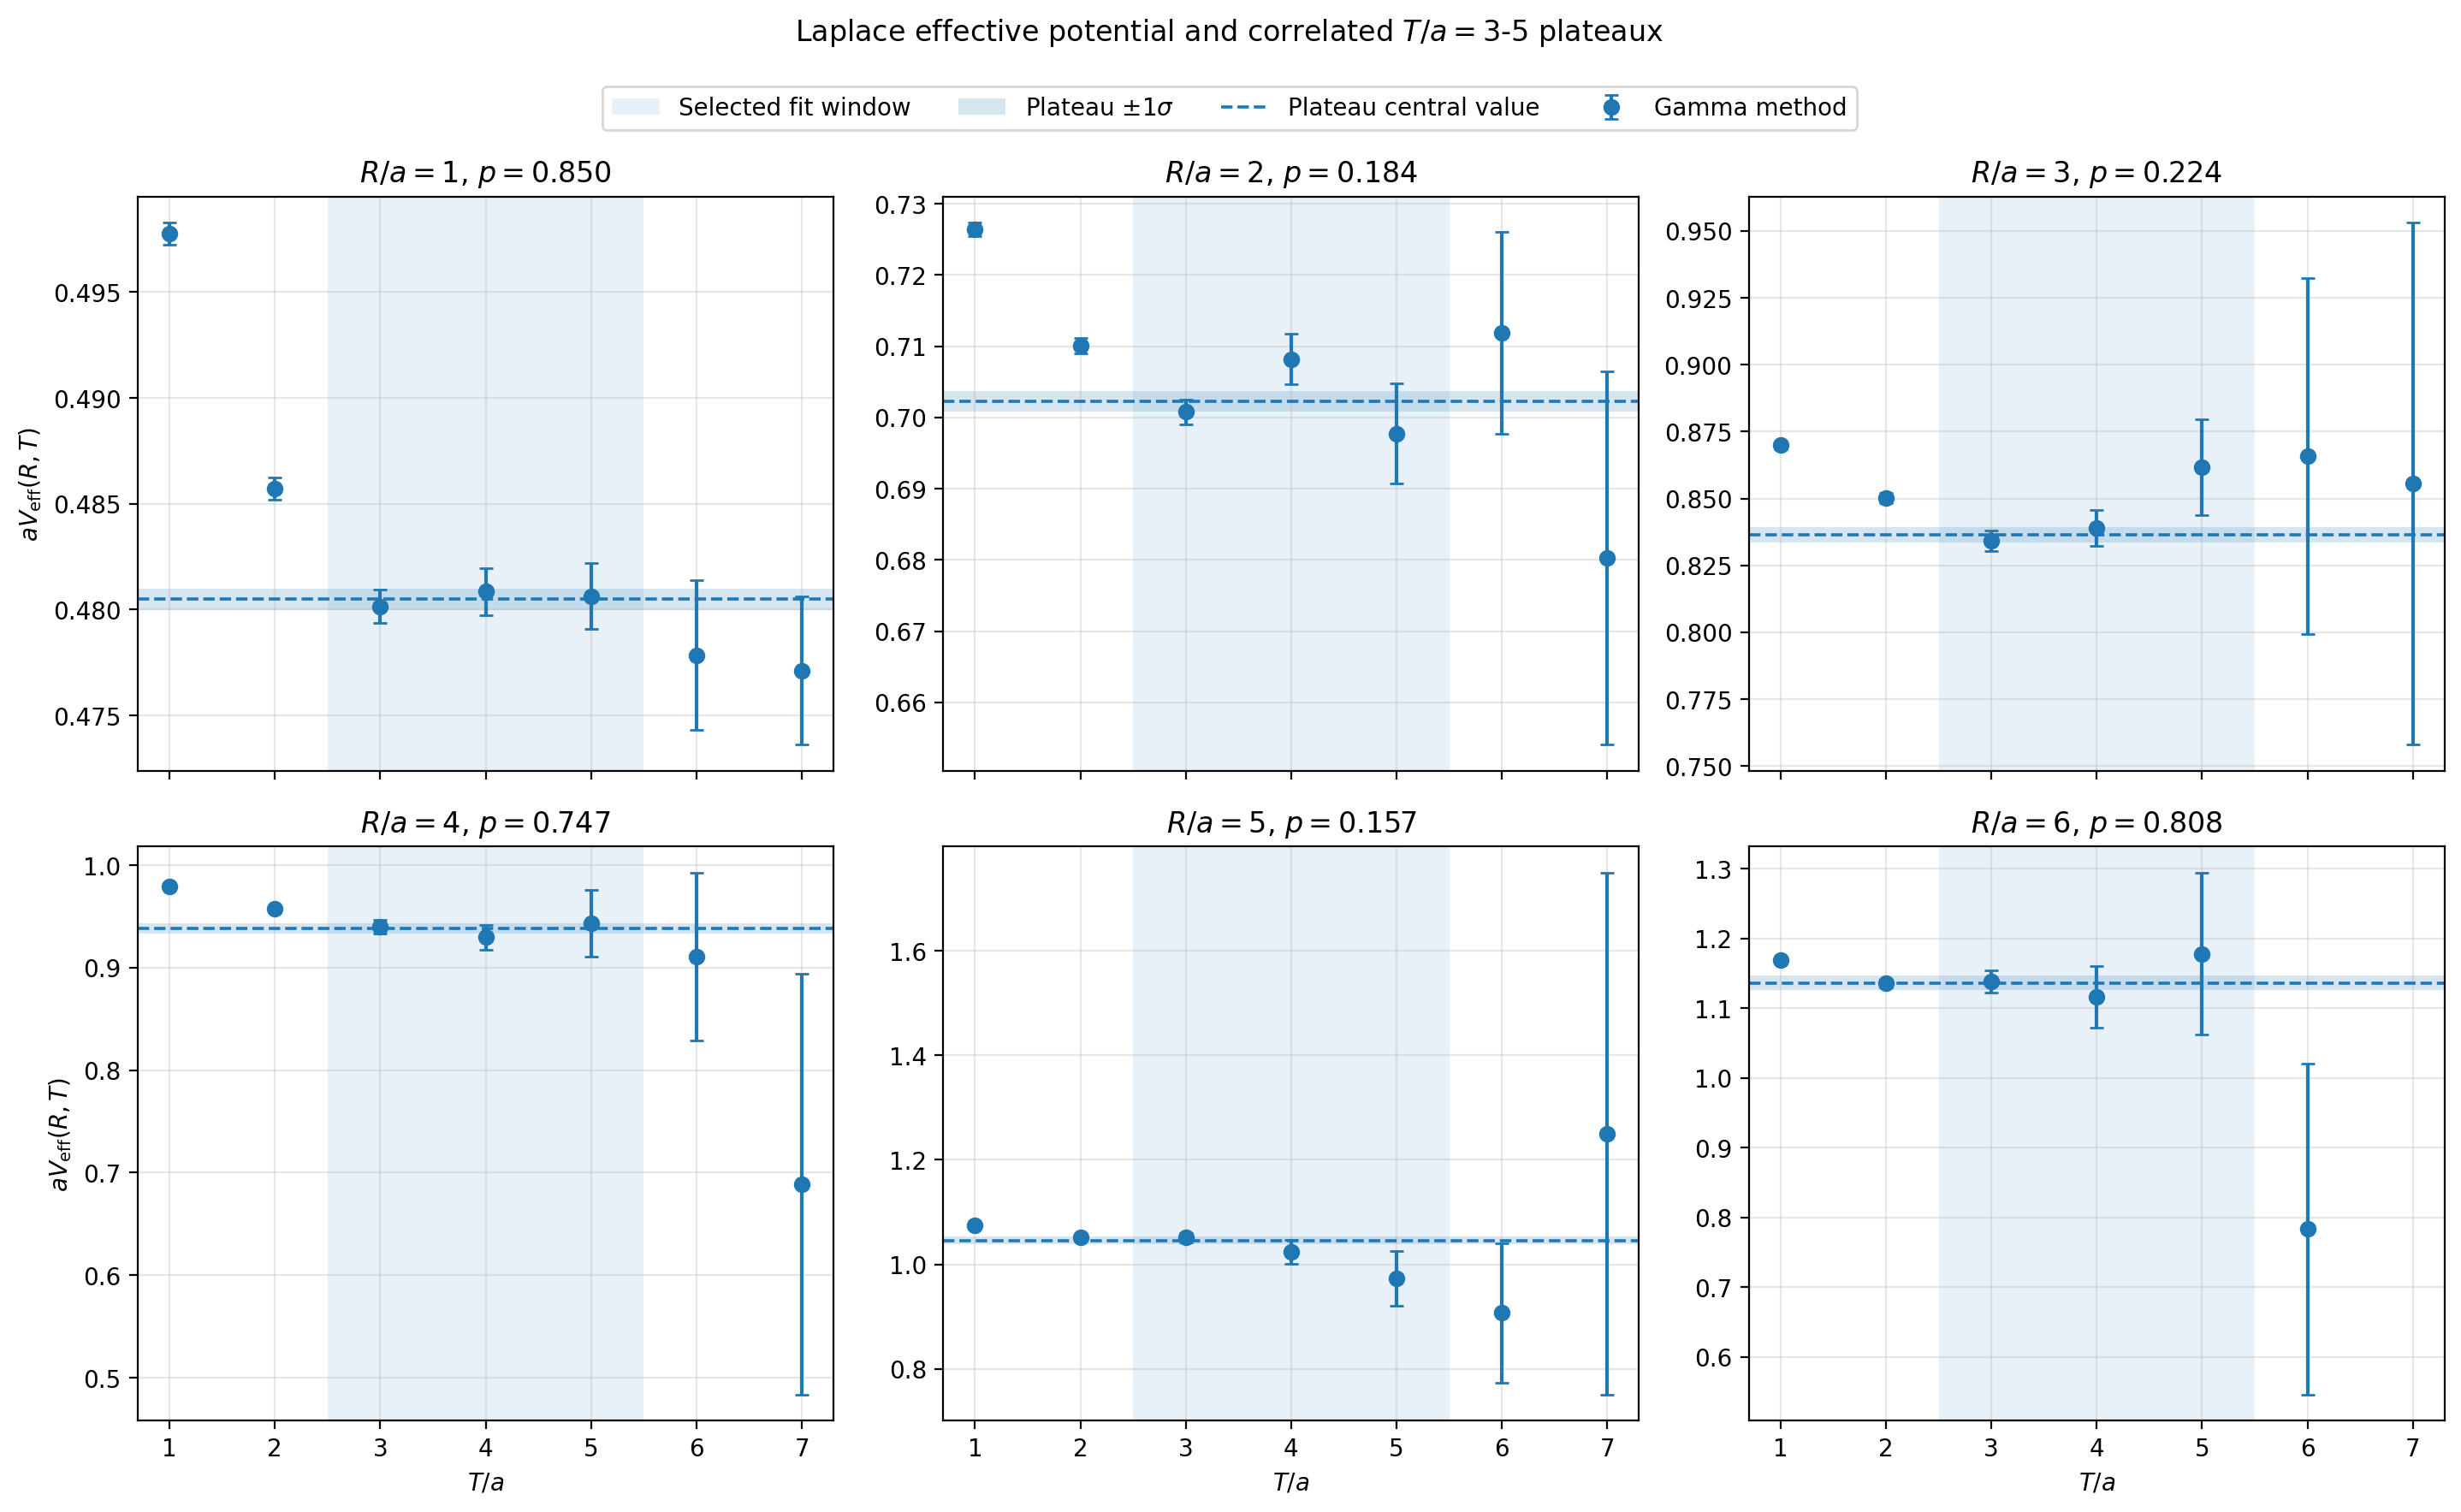
\includegraphics[width=0.95\textwidth]{figures/laplace_Veff_correlated_plateau_T3-5_t0avg6_R1-6.png}
  \caption{\prelim{} correlated plateau analysis for \(R/a=1,\ldots,6\) using temporal-source averaging. The highlighted window \(\tau/a=3,4,5\) is used for the benchmark static-potential extraction.}
  \label{fig:plateaus-r1-r6}
\end{figure}

\section{Cornell fit}
The plateau values are fitted to the Cornell form in \cref{eq:cornell}. The current benchmark fit gives
\begin{align}
  aV_0 &= 0.6646(82), & \sigma a^2 &= 0.08646(24), & \alpha &= 0.2705(60),
\end{align}
with \(a\sqrt{\sigma}=0.2940(40)\), \(\chi^2/\mathrm{dof}\approx1.11\), and \(p=0.344\). These values should be treated as validation-stage results rather than the final physics output.

\begin{figure}[htbp]
  \centering
  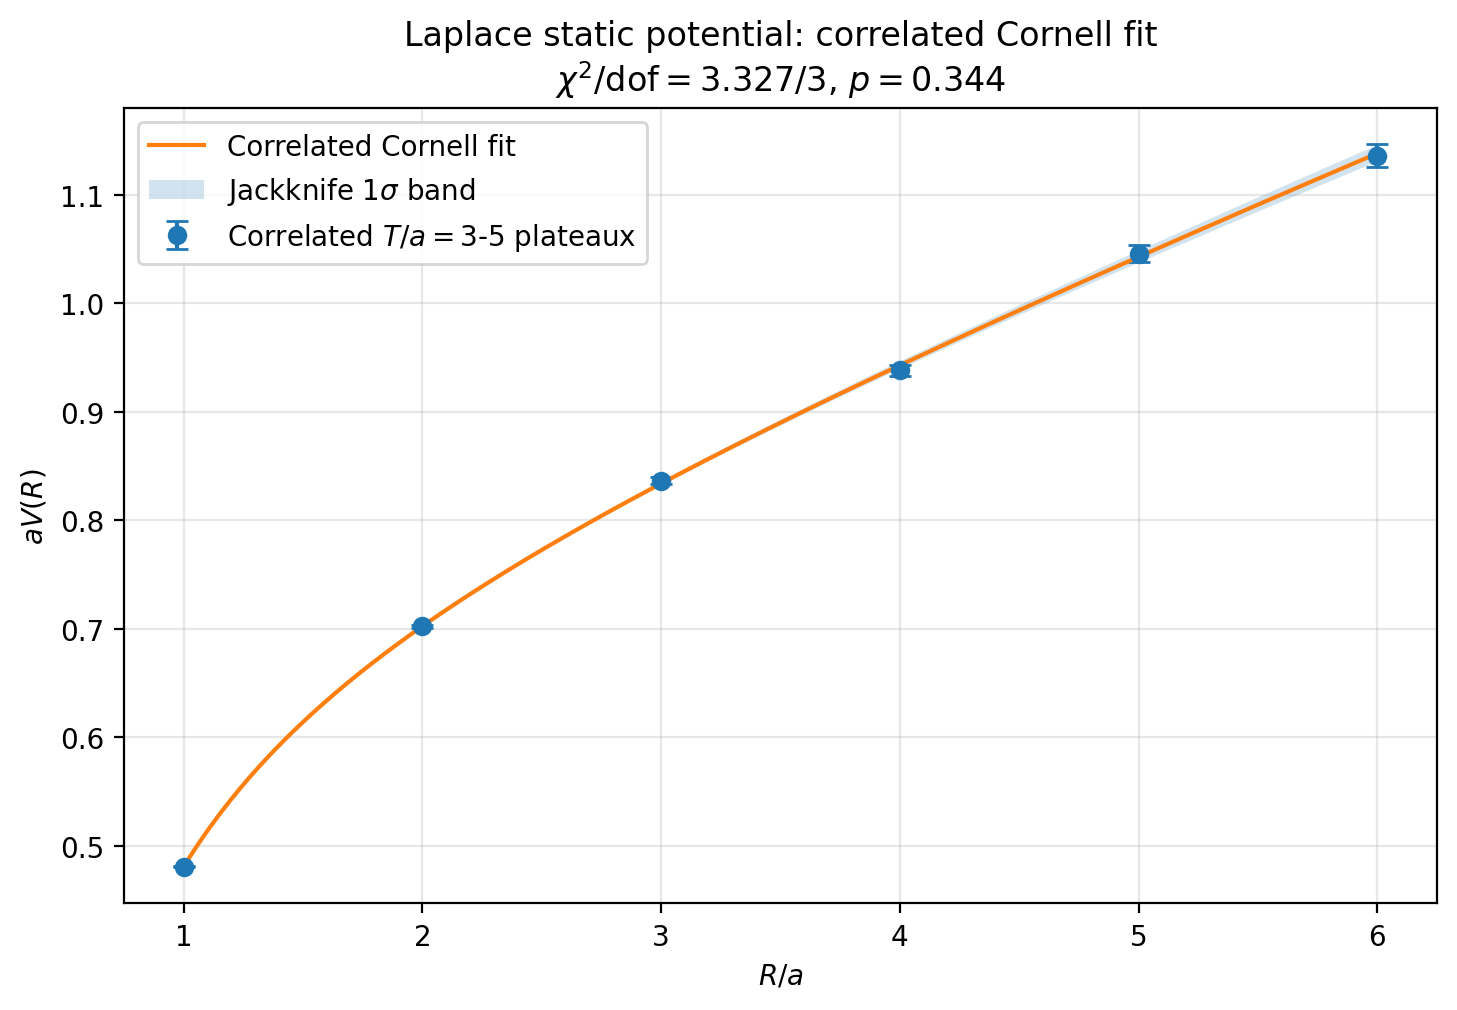
\includegraphics[width=0.78\textwidth]{figures/laplace_static_potential_cornell_R1-6_t0avg6.png}
  \caption{\prelim{} correlated Cornell fit to the validated \(R/a=1,\ldots,6\) static-potential points.}
  \label{fig:cornell-r1-r6}
\end{figure}

\begin{figure}[htbp]
  \centering
  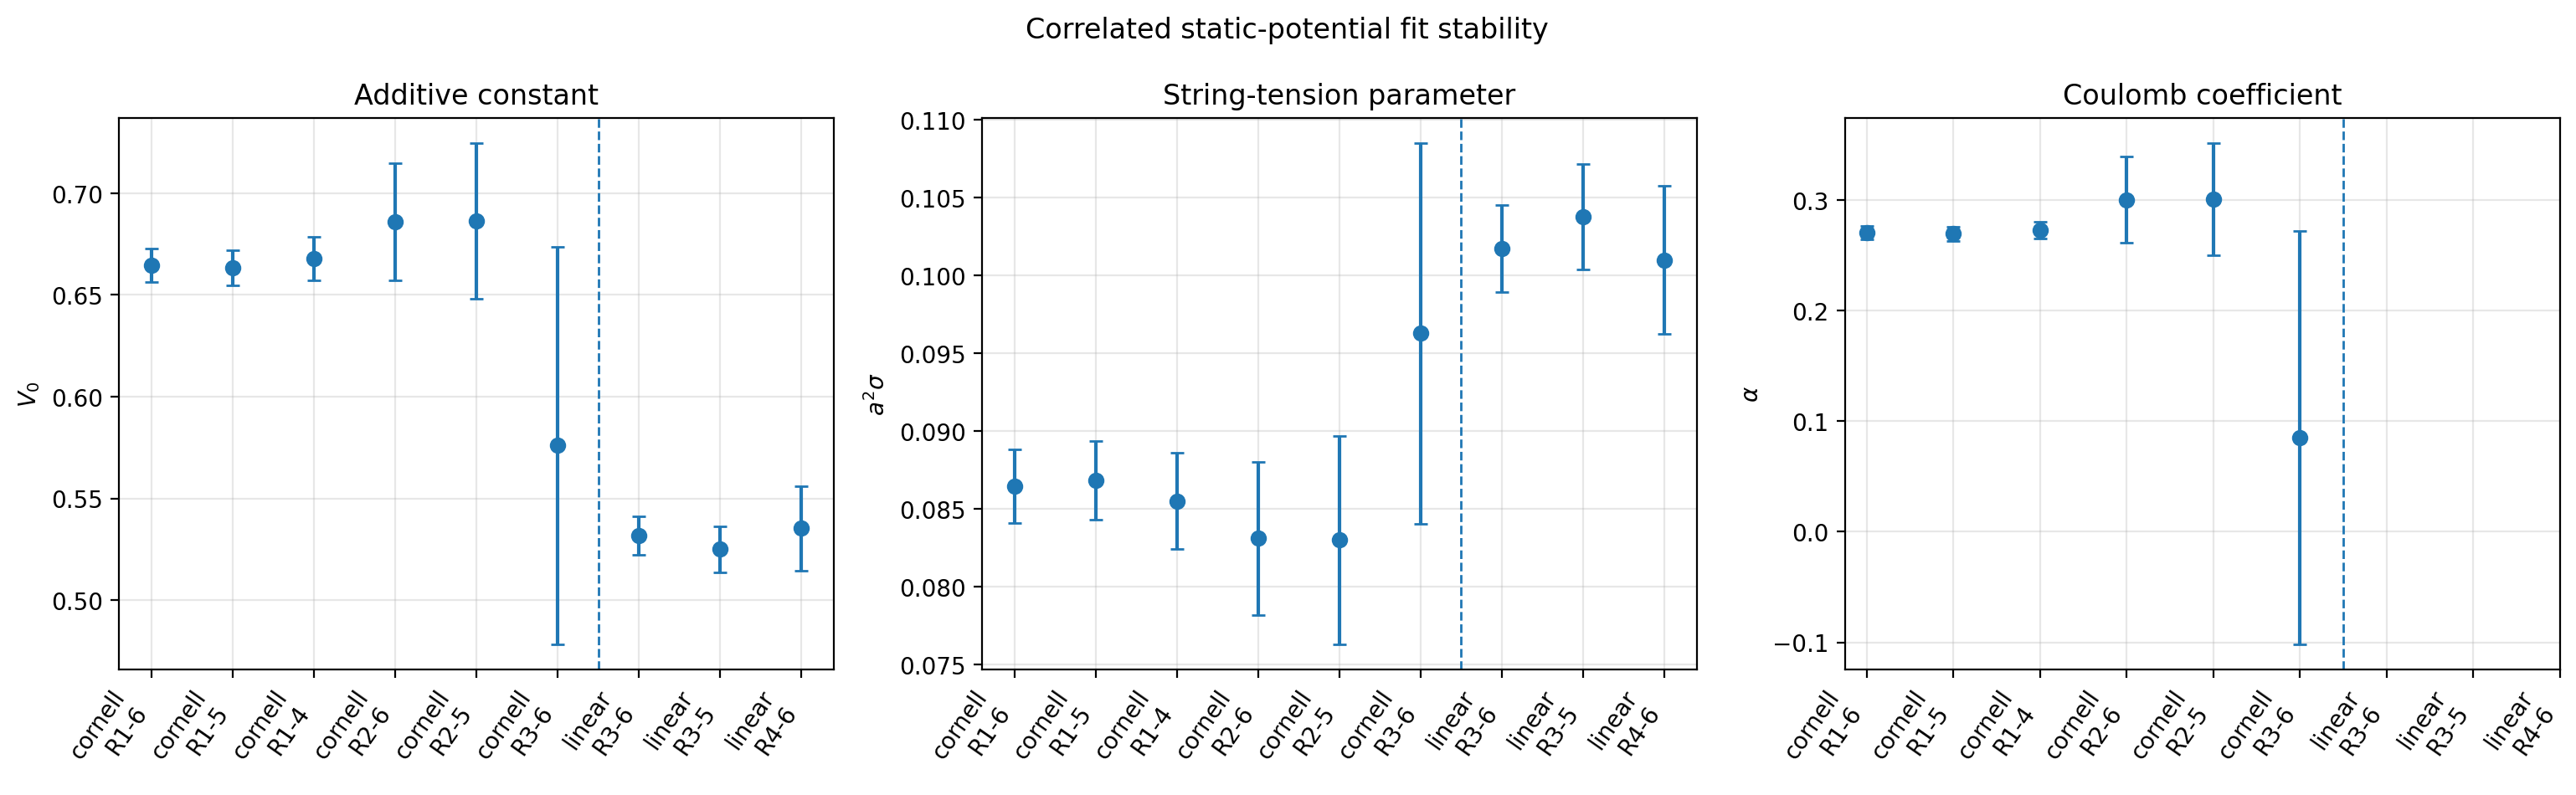
\includegraphics[width=0.78\textwidth]{figures/laplace_static_potential_fit_stability_t0avg6_R6.png}
  \caption{\prelim{} fit-stability diagnostic for the Cornell benchmark. This plot is retained in the thesis draft to document how the chosen fit range was assessed.}
  \label{fig:fit-stability}
\end{figure}

\section{Extended diagnostic scan}
The extended scan probes \(R/a\leq 12\) and \(\tau/a\leq10\). It is not yet used as a final potential extraction at all separations. Instead, it classifies safe, marginal, and diagnostic regions based on relative uncertainty and sign/log stability. \Cref{fig:reliability-diagnostics} shows the current reliability maps.

\begin{figure}[htbp]
  \centering
  \begin{subfigure}{0.32\textwidth}
    \centering
    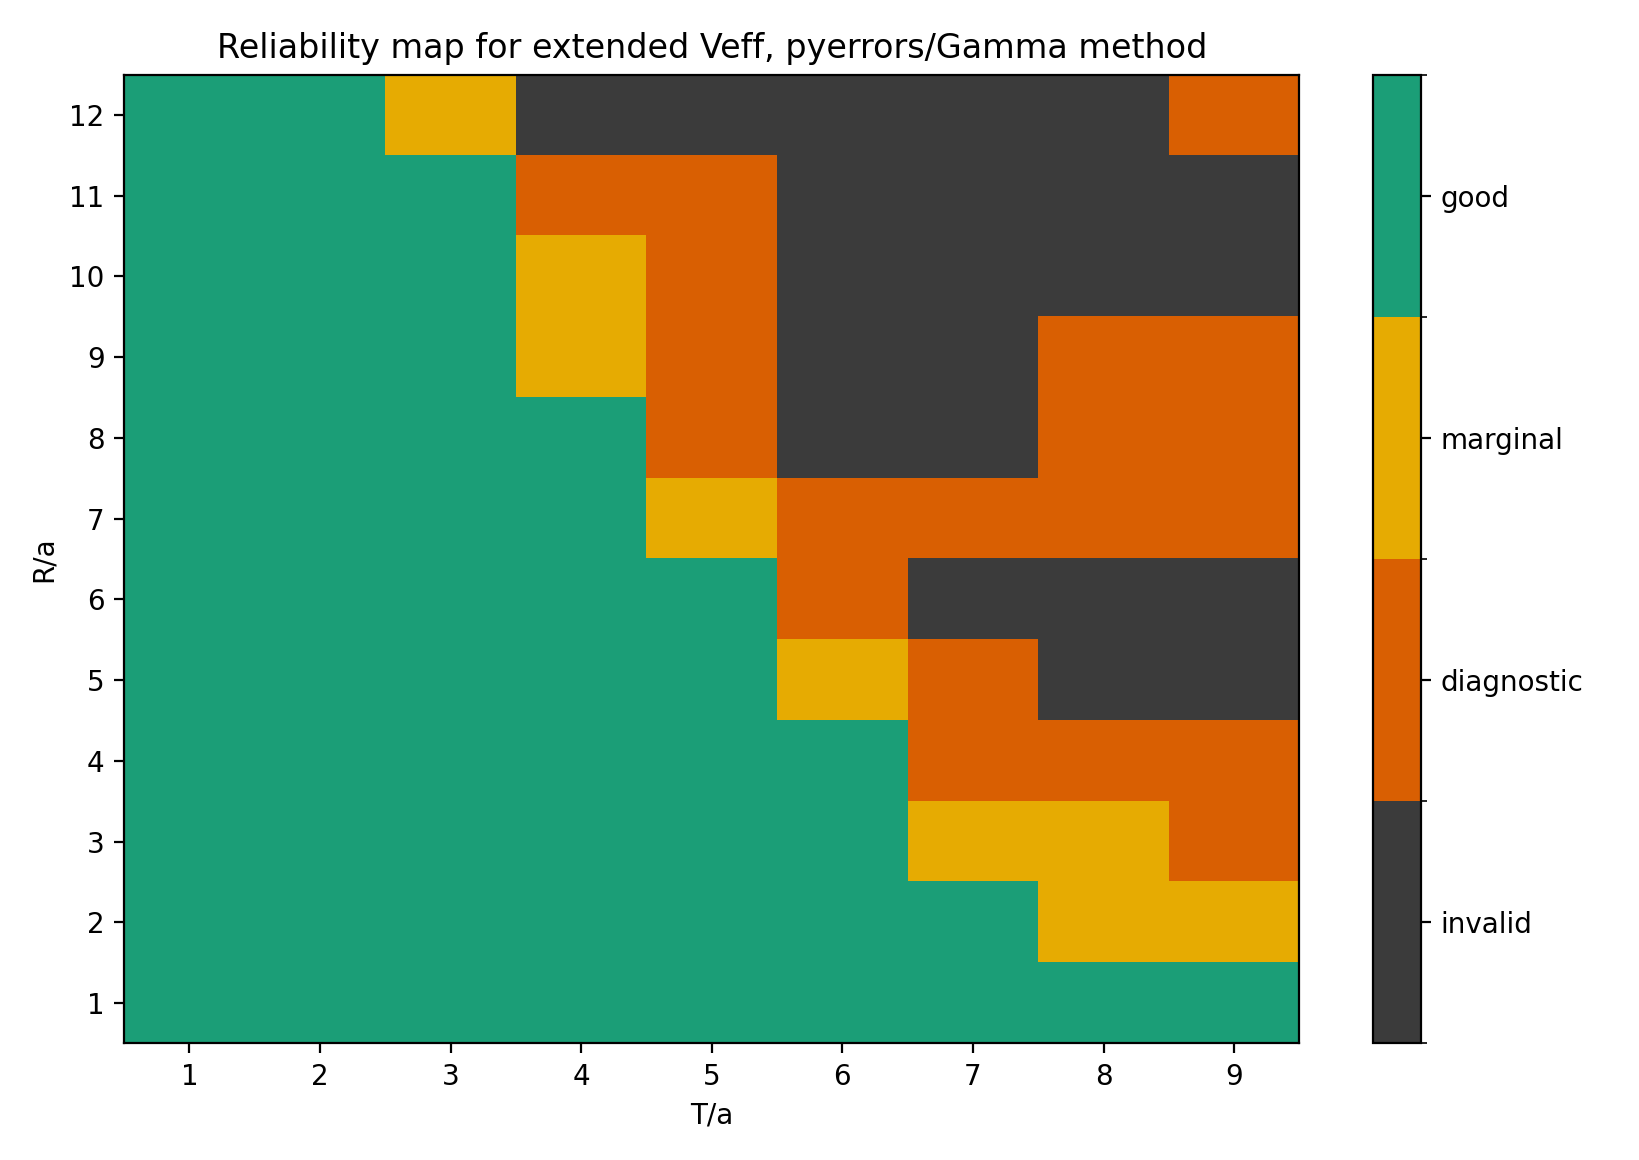
\includegraphics[width=\textwidth]{figures/laplace_reliability_map_t0avg6_R12T10.png}
    \caption{Quality class}
  \end{subfigure}\hfill
  \begin{subfigure}{0.32\textwidth}
    \centering
    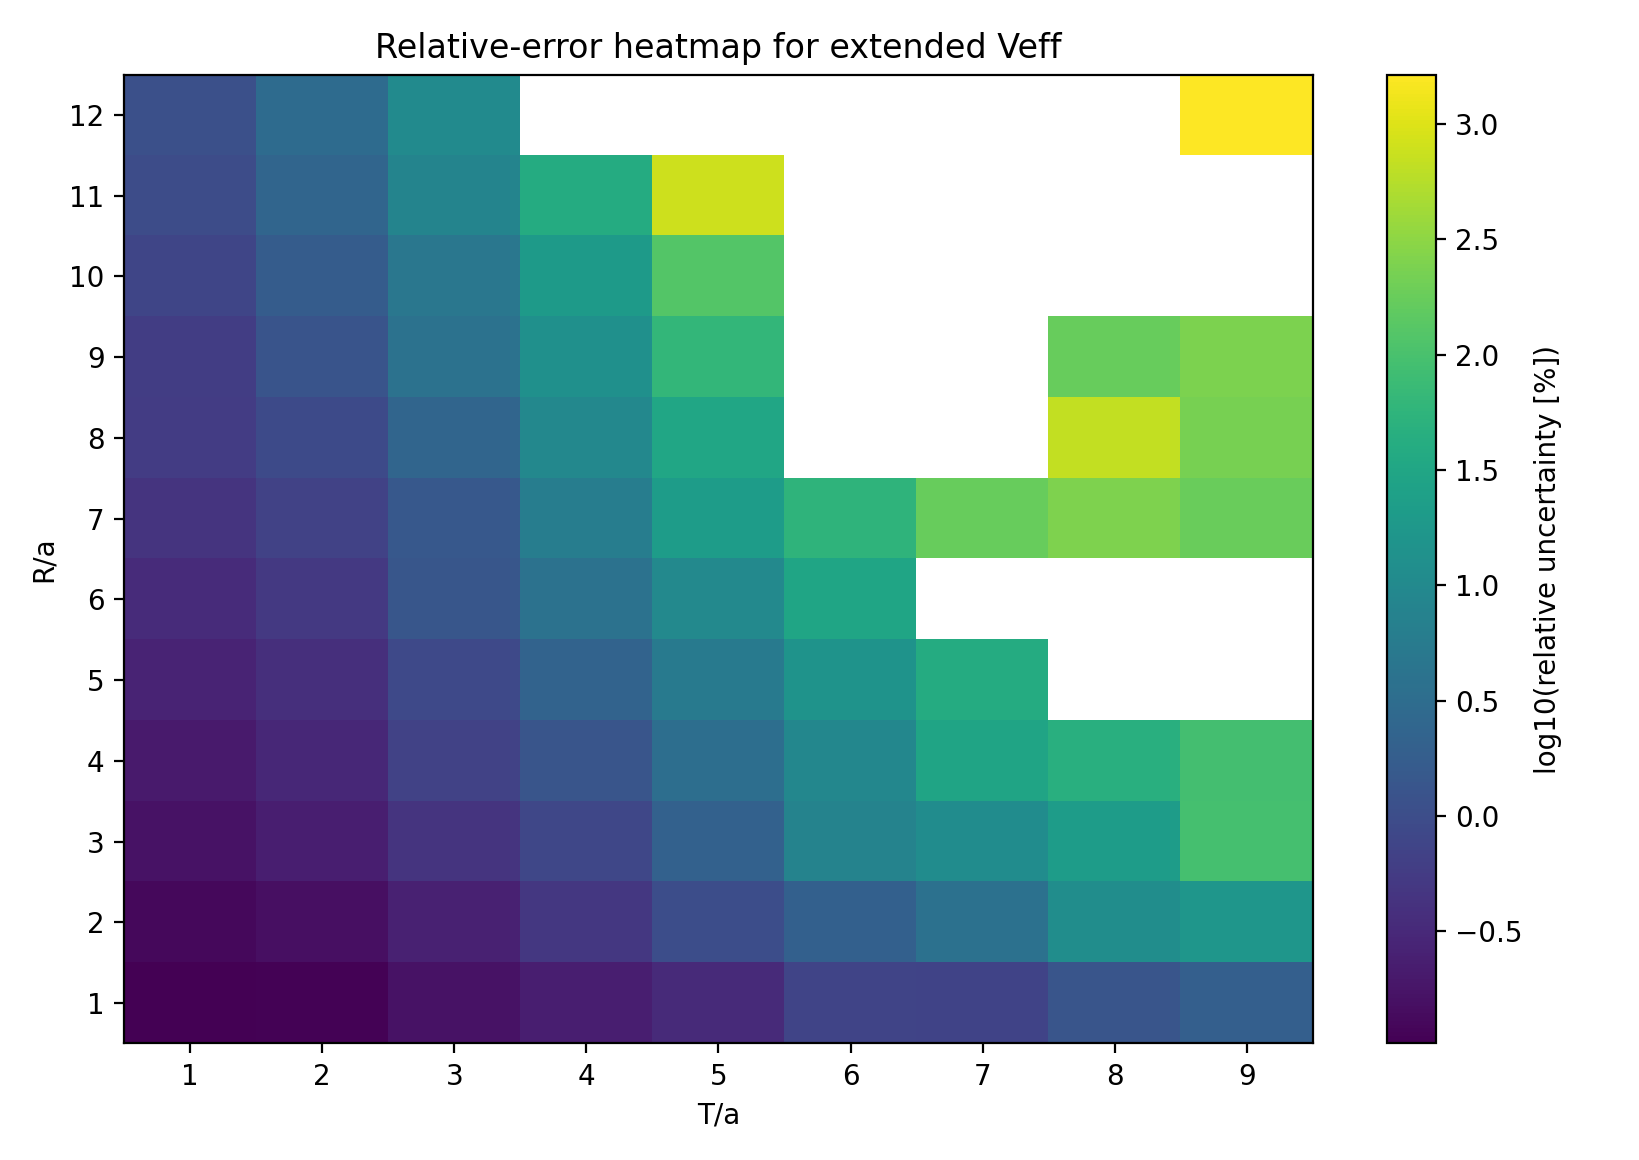
\includegraphics[width=\textwidth]{figures/laplace_relative_error_heatmap_t0avg6_R12T10.png}
    \caption{Relative error}
  \end{subfigure}\hfill
  \begin{subfigure}{0.32\textwidth}
    \centering
    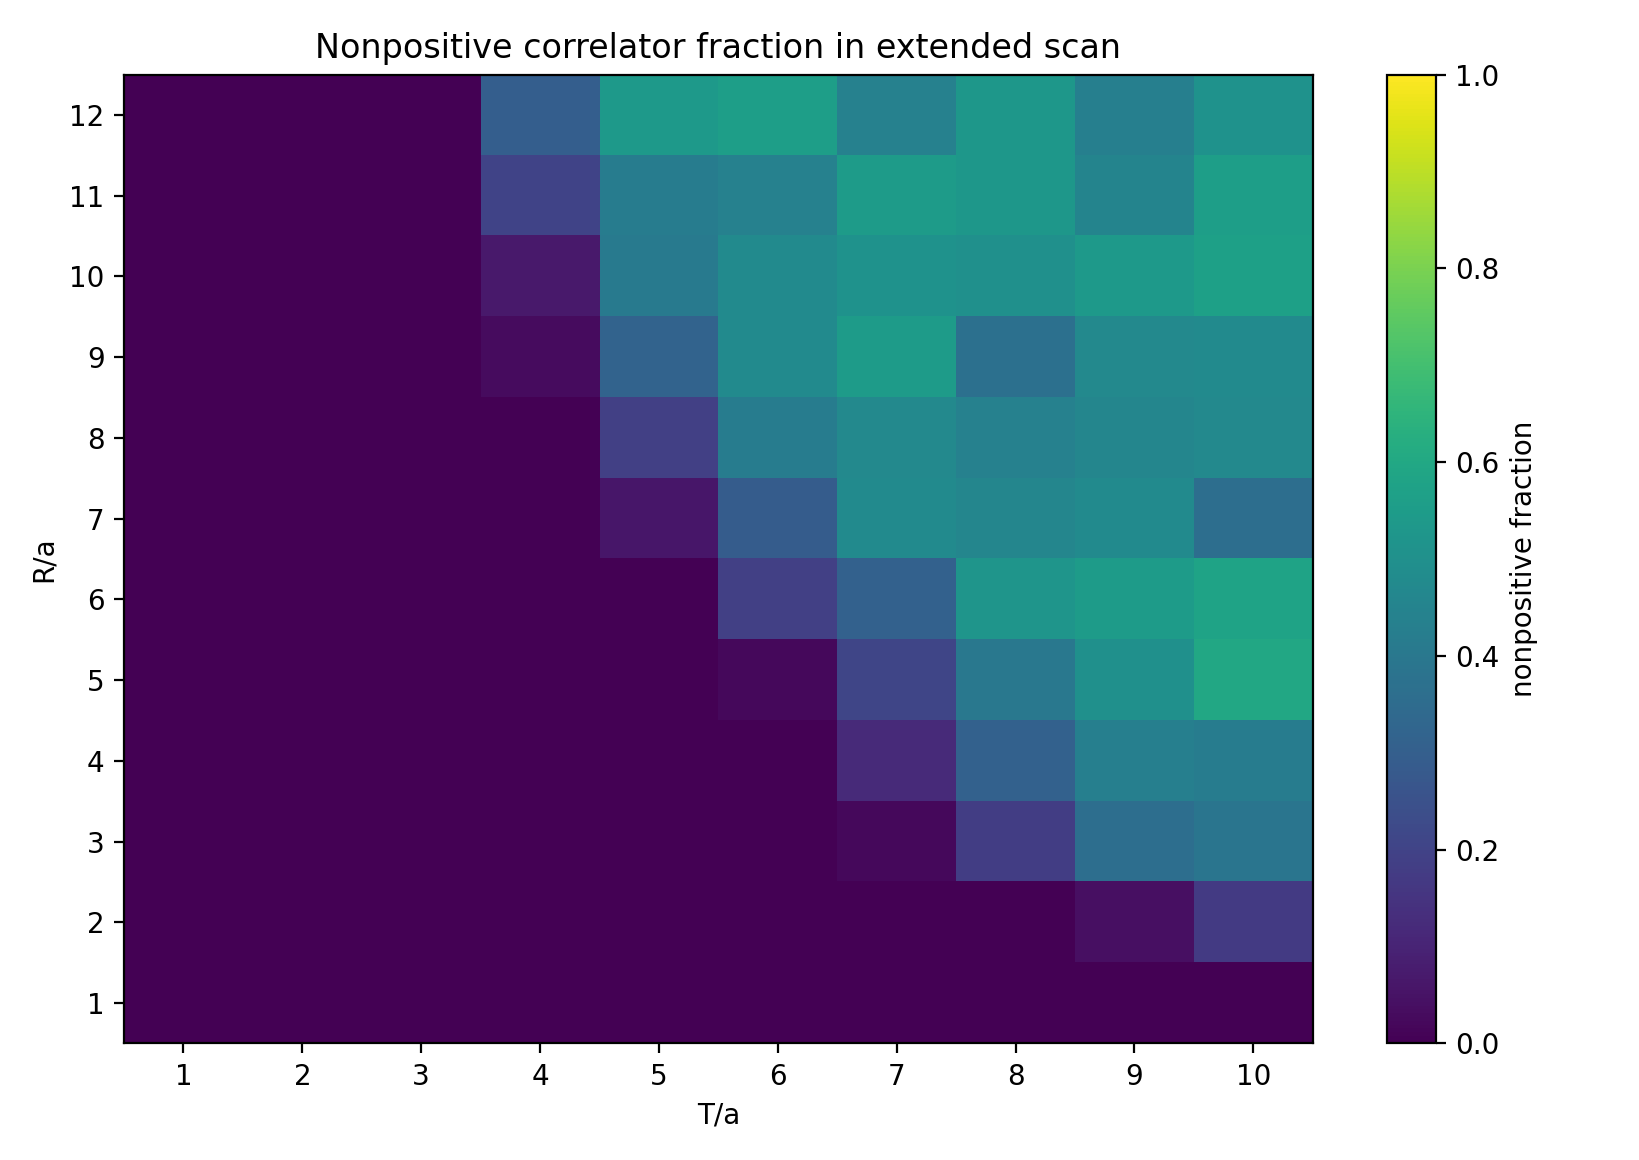
\includegraphics[width=\textwidth]{figures/laplace_nonpositive_fraction_heatmap_t0avg6_R12T10.png}
    \caption{Non-positive fraction}
  \end{subfigure}
  \caption{\prelim{} reliability diagnostics for the extended scan. The maps are used to define safe parameter windows before the flux-tube probe measurements are performed.}
  \label{fig:reliability-diagnostics}
\end{figure}

\begin{figure}[htbp]
  \centering
  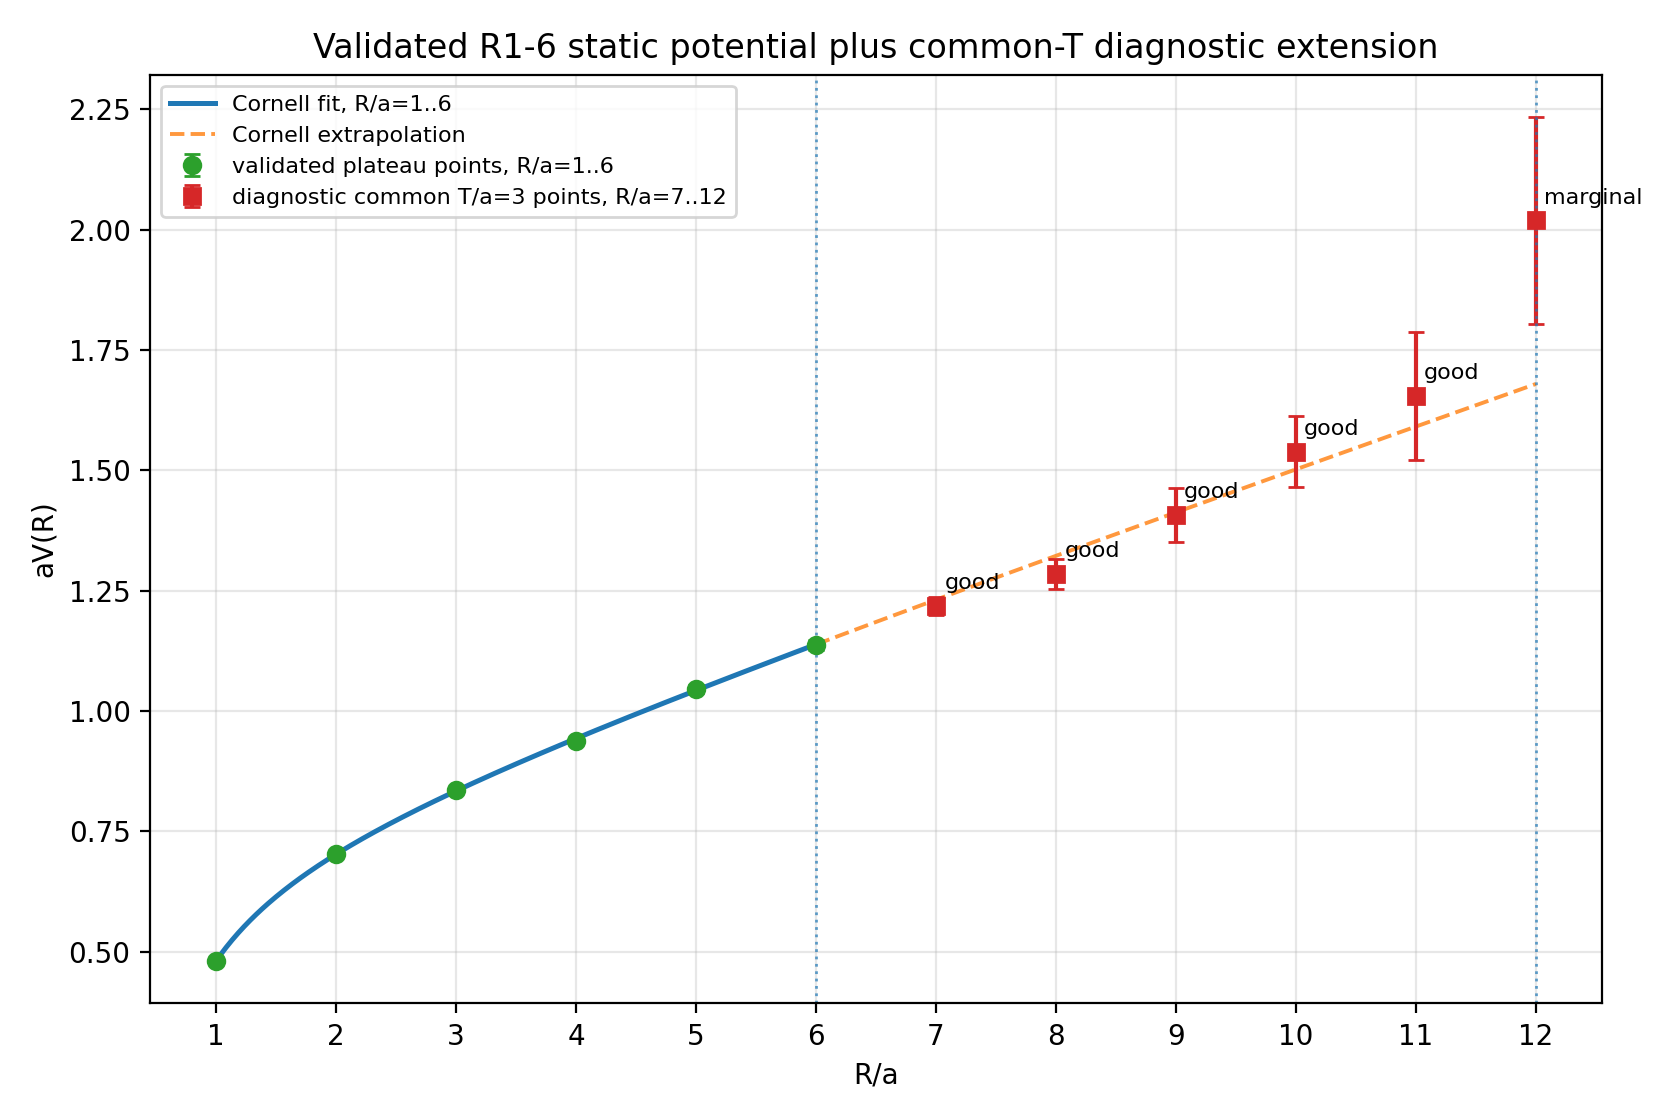
\includegraphics[width=0.80\textwidth]{figures/laplace_static_potential_R1-6_fit_plus_R7-12_commonT3_diagnostic_t0avg6.png}
  \caption{\prelim{} diagnostic extension of the static potential beyond the validated range using a common \(\tau/a=3\) estimate. The larger-\(R\) points are useful for trend checks but are not yet final precision data.}
  \label{fig:potential-diagnostic-extension}
\end{figure}
